\documentclass{article}
\usepackage{graphics} 
\usepackage{hyperref}

\author{Kevin Zollicoffer}
\title{Predictive Modeling\\Lesson 2\\\emph{CART}}
\date{09/23/2013}

\usepackage{Sweave}
\begin{document}
\maketitle
%\tableofcontents
\Sconcordance{concordance:CART.tex:CART.Rnw:%
1 8 1 1 0 11 1 1 2 1 0 2 1 26 0 1 2 2 1 1 2 1 0 5 1 25 0 1 1 26 0 1 2 2 %
1 1 2 1 0 1 1 3 0 1 2 2 1 1 2 1 0 1 1 3 0 2 2 1 0 1 1 3 0 1 2 6 1 1 2 %
22 0 1 2 1 1 1 2 7 0 1 2 8 1 1 2 11 0 1 2 2 1 1 2 22 0 1 2 30 1}


\section*{Introduction}
The RStudio project files and accompanying artifacts, including the tex file that created this PDF, are publicly available on GitHub
\\
\url{https://github.com/zollie/PASS-PredictiveModeling-CART}

\section*{Data Setup}
I took the Excel spreadsheet and saved it as a CSV for easy import into R
\begin{Schunk}
\begin{Sinput}
> wine <- read.csv("~/R/PASS/PredictiveModeling/CART/Wine.csv")
> wine <- wine[1:178,1:14]
> head(wine)
\end{Sinput}
\begin{Soutput}
  Type Alcohol Malic_Acid  Ash Ash_Alcalinity Magnesium Total_Phenols
1    A   14.23       1.71 2.43           15.6       127          2.80
2    A   13.20       1.78 2.14           11.2       100          2.65
3    A   13.16       2.36 2.67           18.6       101          2.80
4    A   14.37       1.95 2.50           16.8       113          3.85
5    A   13.24       2.59 2.87           21.0       118          2.80
6    A   14.20       1.76 2.45           15.2       112          3.27
  Flavanoids Nonflavanoid_Phenols Proanthocyanins Color_Intensity  Hue
1       3.06                 0.28            2.29            5.64 1.04
2       2.76                 0.26            1.28            4.38 1.05
3       3.24                 0.30            2.81            5.68 1.03
4       3.49                 0.24            2.18            7.80 0.86
5       2.69                 0.39            1.82            4.32 1.04
6       3.39                 0.34            1.97            6.75 1.05
  OD280_OD315 Proline
1        3.92    1065
2        3.40    1050
3        3.17    1185
4        3.45    1480
5        2.93     735
6        2.85    1450
\end{Soutput}
\end{Schunk}

\section*{Partitioning}
Next, partition the data into 50\% Train and 50\% Test sets. I set the RNG seed for reproducibility
\begin{Schunk}
\begin{Sinput}
> set.seed(21275)
> n <- nrow(wine)
> nt <- sort(sample(1:n, floor(n/2)))
> train <- wine[nt,]
> test <- wine[-nt,]
> head(train)
\end{Sinput}
\begin{Soutput}
   Type Alcohol Malic_Acid  Ash Ash_Alcalinity Magnesium Total_Phenols
1     A   14.23       1.71 2.43           15.6       127          2.80
6     A   14.20       1.76 2.45           15.2       112          3.27
8     A   14.06       2.15 2.61           17.6       121          2.60
9     A   14.83       1.64 2.17           14.0        97          2.80
10    A   13.86       1.35 2.27           16.0        98          2.98
11    A   14.10       2.16 2.30           18.0       105          2.95
   Flavanoids Nonflavanoid_Phenols Proanthocyanins Color_Intensity  Hue
1        3.06                 0.28            2.29            5.64 1.04
6        3.39                 0.34            1.97            6.75 1.05
8        2.51                 0.31            1.25            5.05 1.06
9        2.98                 0.29            1.98            5.20 1.08
10       3.15                 0.22            1.85            7.22 1.01
11       3.32                 0.22            2.38            5.75 1.25
   OD280_OD315 Proline
1         3.92    1065
6         2.85    1450
8         3.58    1295
9         2.85    1045
10        3.55    1045
11        3.17    1510
\end{Soutput}
\begin{Sinput}
> head(test)
\end{Sinput}
\begin{Soutput}
   Type Alcohol Malic_Acid  Ash Ash_Alcalinity Magnesium Total_Phenols
2     A   13.20       1.78 2.14           11.2       100          2.65
3     A   13.16       2.36 2.67           18.6       101          2.80
4     A   14.37       1.95 2.50           16.8       113          3.85
5     A   13.24       2.59 2.87           21.0       118          2.80
7     A   14.39       1.87 2.45           14.6        96          2.50
12    A   14.12       1.48 2.32           16.8        95          2.20
   Flavanoids Nonflavanoid_Phenols Proanthocyanins Color_Intensity  Hue
2        2.76                 0.26            1.28            4.38 1.05
3        3.24                 0.30            2.81            5.68 1.03
4        3.49                 0.24            2.18            7.80 0.86
5        2.69                 0.39            1.82            4.32 1.04
7        2.52                 0.30            1.98            5.25 1.02
12       2.43                 0.26            1.57            5.00 1.17
   OD280_OD315 Proline
2         3.40    1050
3         3.17    1185
4         3.45    1480
5         2.93     735
7         3.58    1290
12        2.82    1280
\end{Soutput}
\end{Schunk}

\section*{CART with the rpart package}
First we build the decision tree with train data
\begin{Schunk}
\begin{Sinput}
> library(rpart)
> fit <- rpart(Type ~ ., data=train, method="class", minbucket = 1)
\end{Sinput}
\end{Schunk}

\noindent
Then make predictions using the test data
\begin{Schunk}
\begin{Sinput}
> pred <- predict(fit, newdata=test, type="class")
> tab <- table(pred, test[,"Type"]) 
\end{Sinput}
\end{Schunk}
Visually the tree looks like
\begin{Schunk}
\begin{Sinput}
> library(rpart.plot)
> prp(fit)
\end{Sinput}
\end{Schunk}

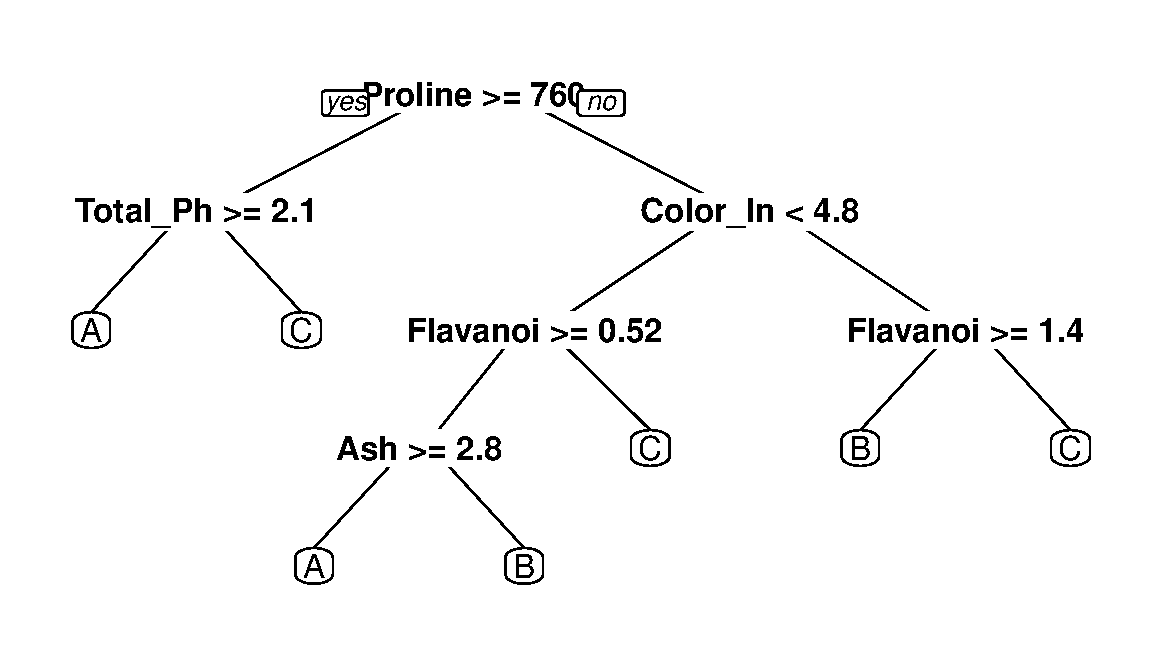
\includegraphics[width=0.98\textwidth]{rpart-fit-prp-default.pdf}


\section*{Lesson 2 Question and Answer}
\subsection*1\emph{What is the error rate for the validation data?}

\begin{Schunk}
\begin{Sinput}
> printcp(fit)
\end{Sinput}
\begin{Soutput}
Classification tree:
rpart(formula = Type ~ ., data = train, method = "class", minbucket = 1)

Variables actually used in tree construction:
[1] Flavanoids  Hue         Magnesium   OD280_OD315 Proline    

Root node error: 53/89 = 0.59551

n= 89 

        CP nsplit rel error  xerror     xstd
1 0.566038      0  1.000000 1.20755 0.080000
2 0.320755      1  0.433962 0.45283 0.078994
3 0.037736      2  0.113208 0.20755 0.058583
4 0.018868      4  0.037736 0.16981 0.053666
5 0.010000      5  0.018868 0.20755 0.058583
\end{Soutput}
\end{Schunk}
\noindent 
The error rate is 
\begin{Schunk}
\begin{Sinput}
> 1-sum(diag(tab))/sum(tab)
\end{Sinput}
\begin{Soutput}
[1] 0.1460674
\end{Soutput}
\end{Schunk}

\noindent

\subsection*2\emph{Indicate the number of misclassification}
\newline
\newline
\noindent
The Classification Matrix is given below

\begin{Schunk}
\begin{Sinput}
> tab
\end{Sinput}
\begin{Soutput}
pred     A  B  C
      0  0  0  0
   A  0 25  2  6
   B  0  1 31  2
   C  0  0  2 20
\end{Soutput}
\end{Schunk}

\subsection*3\emph{Study the Best Pruned tree and develop a set of classification rules, using if-then statement; e.g. "if a >= b then A" and "if a < b then B" }

\begin{Schunk}
\begin{Sinput}
> fit
\end{Sinput}
\begin{Soutput}
n= 89 

node), split, n, loss, yval, (yprob)
      * denotes terminal node

 1) root 89 53 B (0.00000000 0.37078652 0.40449438 0.22471910)  
   2) Proline>=755 34  2 A (0.00000000 0.94117647 0.05882353 0.00000000)  
     4) Magnesium< 133.5 32  0 A (0.00000000 1.00000000 0.00000000 0.00000000) *
     5) Magnesium>=133.5 2  0 B (0.00000000 0.00000000 1.00000000 0.00000000) *
   3) Proline< 755 55 21 B (0.00000000 0.01818182 0.61818182 0.36363636)  
     6) OD280_OD315>=2.185 32  1 B (0.00000000 0.03125000 0.96875000 0.00000000) *
     7) OD280_OD315< 2.185 23  3 C (0.00000000 0.00000000 0.13043478 0.86956522)  
      14) Hue>=0.965 2  0 B (0.00000000 0.00000000 1.00000000 0.00000000) *
      15) Hue< 0.965 21  1 C (0.00000000 0.00000000 0.04761905 0.95238095)  
        30) Flavanoids>=1.475 1  0 B (0.00000000 0.00000000 1.00000000 0.00000000) *
        31) Flavanoids< 1.475 20  0 C (0.00000000 0.00000000 0.00000000 1.00000000) *
\end{Soutput}
\end{Schunk}

\noindent
If Proline greater than or equal to 760 and Color greater than or equal to 4.8 and Flavanoids greater than or equal to 1.4 then C
\\
\\
\noindent
If Proline greater than or equal to 760 and Color greater than or equal to 4.8 and Flavanoids less than 1.4 then B
\\
\\
\noindent
If Proline greater than or equal to 760 and Color less than 4.8 and Flavanoids greater than or equal to .52 then C
\\
\\
\noindent
If Proline greater than or equal to 760 and Color less than 4.8 and Flavanoids less than .52 and Ash greater than or equal to 2.8 then B
\\
\\
\noindent
If Proline greater than or equal to 760 and Color less than 4.8 and Flavanoids less than .52 and Ash less than 2.8 then A
\\
\\
\noindent
If Proline less than 760 and  Total Phenols greater than or equal to 2.1 then C
\\
\\
\noindent
If Proline less than 760 and  Total Phenols less than 2.1 then A
\end{document}



